% !TEX program = pdflatex
\documentclass[letterpaper,12pt]{article}
\usepackage[utf8]{inputenc}
\usepackage[spanish,mexico]{babel}
\usepackage[T1]{fontenc}
\usepackage{lmodern,amsmath,amssymb}
\usepackage{graphicx,float,xcolor,array,booktabs,tabularx,ragged2e}
\usepackage{tikz}
\usetikzlibrary{arrows.meta,positioning,calc}
\usepackage{listings}
\usepackage[left=25mm,right=25mm,top=30mm,bottom=25mm,headheight=15pt]{geometry}
\usepackage{parskip,fancyhdr,pdflscape,microtype}
\usepackage{hyperref}
\graphicspath{{img/}{portada_img/}}
\newcommand{\materia}{Laboratorio de Organización y Arquitectura de Computadoras}
\pagestyle{fancy}
\fancyhf{}
\fancyhead[R]{\small\textsc{\materia}}
\fancyfoot[C]{\thepage}
\renewcommand{\headrulewidth}{0.8pt}
\hypersetup{colorlinks=true,linkcolor=blue!55!black,urlcolor=blue!55!black,
 pdftitle={Práctica 7. Procesador CISC 68HC11},
 pdfauthor={Espinoza Matamoros Percival Ulises; Montiel Juárez Oscar Iván; Veraza García Amy Valentina}}
\definecolor{codebg}{rgb}{0.96,0.96,0.96}
\definecolor{keyword}{rgb}{0.0,0.2,0.6}
\definecolor{comment}{rgb}{0.20,0.40,0.28}
\definecolor{codegray}{rgb}{0.5,0.5,0.5}
\lstdefinestyle{estiloVHDL}{language=VHDL,basicstyle=\ttfamily\scriptsize,
 backgroundcolor=\color{codebg},commentstyle=\color{comment}\itshape,
 keywordstyle=\color{keyword}\bfseries,numbers=left,
 numberstyle=\tiny\color{codegray},frame=single,breaklines=true,
 breakatwhitespace=false,columns=fullflexible,
 literate={á}{{\'a}}1 {é}{{\'e}}1 {í}{{\'i}}1 {ó}{{\'o}}1 {ú}{{\'u}}1 {ñ}{{\~n}}1
 {Á}{{\'A}}1 {É}{{\'E}}1 {Í}{{\'I}}1 {Ó}{{\'O}}1 {Ú}{{\'U}}1 {Ñ}{{\~N}}1,
 keepspaces=true,showstringspaces=false,tabsize=2,
 xleftmargin=4mm,framexleftmargin=1mm,aboveskip=9pt,belowskip=8pt}
\lstdefinestyle{mif}{style=estiloVHDL,language={},morecomment=[l]{--},numbers=none}
\newcommand{\hx}[1]{\texttt{#1}}
\newcolumntype{Y}{>{\RaggedRight\arraybackslash}X}
\setlength{\emergencystretch}{2em}
\begin{document}
\renewcommand{\lstlistingname}{Código}
\thispagestyle{empty} % Sin encabezado ni pie en la portada

% --- ENCABEZADO DE PORTADA (TABLA DE 3 COLUMNAS) ---
\begin{center}
    % La tabla usa 'm' para centrar verticalmente las imágenes y el texto
    \begin{tabular}{m{0.15\textwidth} m{0.60\textwidth} m{0.15\textwidth}}
        % Logo Izquierdo (UNAM)
        
\includegraphics[width=2cm]{portada_img/escudounam_negro.jpg} & 
        
        % Título Central
        \centering\Huge\textbf{Universidad Nacional Autónoma de México} &
        
        % Logo Derecho (Facultad)
        \raggedleft
\includegraphics[width=2cm]{portada_img/escudofi_negro.jpg}
    \end{tabular}
\end{center}

\vspace{0.3cm}

% --- INFORMACIÓN DEL REPORTE ---
\begin{center}
    {\LARGE \textbf{Facultad de Ingeniería}}\\[1cm]

    {\LARGE \textbf{Laboratorio de Arquitectura y Organización de Computadoras}} \\[1cm]

	{\LARGE Grupo: 07 - Semestre: 2027-1} \\[1cm]
    
    {\LARGE \textbf{Reporte Práctica 7.}}\\[0.5cm]
    {\LARGE Procesador CISC 68HC11}\\[1cm]

    {\Large \textbf{Fecha de Entrega}}\\[0.2cm]
    {\Large 13 de Octubre del 2026} \\[1cm]

    {\LARGE \textbf{Profesor}}\\[0.2cm]
    {\Large Ing. Julio Cesar Cruz Estrada}\\[1cm]
    
    {\LARGE \textbf{Integrantes:}}\\[0.2cm]
    {\Large Espinoza Matamoros Percival Ulises}\\[0.5cm]
    {\Large Montiel Juárez Oscar Iván}\\[0.5cm]
    {\Large Veraza García Amy Valentina}\\[0.5cm]

\end{center}

\clearpage

\section{Objetivo}
Analizar y ampliar el funcionamiento de un procesador CISC de 8 bits basado en el 68HC11, mediante la preparación de su memoria de microprograma y la ejecución de programas en lenguaje máquina. Verificar en simulación las cargas de datos, la suma de acumuladores, la comparación, los saltos y las transferencias entre registros y memoria.

\section{Introducción}
Una instrucción del procesador requiere varias operaciones internas: colocar una dirección en el bus, leer un dato, seleccionar los operandos de la unidad de procesamiento aritmético (UPA), guardar el resultado y actualizar las banderas. En el proyecto utilizado, estas operaciones se coordinan mediante palabras de control almacenadas en la memoria del secuenciador.

La práctica se desarrolló a partir del proyecto base y de los materiales de apoyo del profesor. Se trabajó en dos niveles: la microprogramación define cómo se ejecuta cada instrucción y el código máquina determina qué instrucciones ejecuta el procesador. Se presentan tres ejercicios y seis pruebas: suma repetitiva y carga de \hx{FF}, comparación de registros con valores iguales y diferentes, y comparación con acceso a memoria en ambos casos.

\section{Desarrollo}
\subsection{Organización del procesador}
La arquitectura dispone de dos acumuladores de 8 bits, $A$ y $B$, una UPA, un registro de códigos de condición (CCR), un contador de programa (PC), registros auxiliares y una unidad de control microprogramada. Los datos ocupan bytes de 8 bits y las direcciones que manejan el PC y los saltos extendidos tienen 16 bits. La RAM implementada contiene 256 posiciones de 8 bits; los programas utilizan el intervalo \hx{0000} a \hx{00FF}.

El PC indica la dirección del programa en RAM. La señal \texttt{Edo\_Pres} indica la dirección de la microinstrucción dentro del secuenciador. Son direcciones distintas: el PC avanza según los bytes de la instrucción, mientras que el secuenciador recorre los pasos necesarios para ejecutarla.

\begin{figure}[H]
\centering
\begin{tikzpicture}[font=\small,
 block/.style={draw,rounded corners=2pt,align=center,minimum height=12mm,text width=33mm},
 arrow/.style={-{Latex[length=2mm]},thick}]
\node[block] (ram) at (0,0) {RAM de programa\\\texttt{mem\_content.mif}};
\node[block] (ri) at (5.0,0) {Registro de\\instrucciones};
\node[block] (rom) at (10.0,0) {Memoria de control\\\texttt{memory.vhd}};
\node[block] (pc) at (0,-2.0) {Contador de\\programa (PC)};
\node[block] (seq) at (5.0,-2.0) {Secuenciador\\y selección de prueba};
\node[block] (path) at (10.0,-2.0) {Acumuladores, UPA\\y banderas};
\draw[arrow] (pc) -- (ram) node[midway,left,font=\scriptsize] {dirección};
\draw[arrow] (ram) -- (ri) node[midway,above,font=\scriptsize] {opcode};
\draw[arrow] (ri) -- (rom) node[midway,above,font=\scriptsize] {opcode $\Vert$ \hx{0}};
\draw[arrow] (seq.north east) -- (rom.south west);
\draw[arrow] (rom) -- (path) node[midway,right,font=\scriptsize] {control};
\draw[arrow] (path) -- (seq) node[midway,above,font=\scriptsize] {condiciones};
\draw[arrow] (seq) -- (pc) node[midway,above,font=\scriptsize] {control};
\end{tikzpicture}
\caption{Esquema funcional simplificado de la relación entre programa, microprograma y ruta de datos. Se omiten buses y conexiones auxiliares para destacar el flujo de control.}
\label{fig:arquitectura}
\end{figure}

\subsection{Memoria de programa y memoria de control}
El archivo \texttt{mem\_content.mif} inicializa la RAM declarada en \texttt{RAM/ram.vhd}. Cada posición contiene un opcode, un operando o un dato. Su enlace se establece con el atributo siguiente:
\begin{lstlisting}[style=estiloVHDL,numbers=none]
attribute ram_init_file : string;
attribute ram_init_file of mem : signal is "mem_content.mif";
\end{lstlisting}
El archivo \texttt{Secuenciador/memory.vhd} contiene la memoria de microprograma. Recibe una dirección de 12 bits y entrega una palabra de 98 bits mediante condiciones \texttt{if/elsif}. Cambiar el MIF modifica el programa; cambiar esta memoria modifica las operaciones internas de las instrucciones.

\subsection{Preparación de la microprogramación con la hoja del profesor}
Para preparar las palabras de control se utilizó como referencia el archivo \nolinkurl{salidas_68HC11_CISC-practica7.xlsx}, proporcionado por el profesor \cite{hoja}. La hoja \texttt{salidas} reúne las microdirecciones y las señales de cada palabra. Las columnas separan los campos del secuenciador, los acumuladores, la UPA, los registros, la memoria, las interrupciones y el CCR. La columna final, \texttt{CW}, concatena los valores de cada fila para formar la cadena de 98 bits que se coloca en \texttt{memory.vhd}.

La hoja \texttt{entradas} relaciona las condiciones con los códigos del campo de prueba; por ejemplo, la bandera $Z$ corresponde a \hx{10010}. Las hojas de instrucciones y de \textit{fetch} relacionan las señales con las transferencias entre registros. También se consultaron los diagramas de direccionamiento inmediato y extendido y la tabla de líneas de control \cite{diagramas,control}.

El procedimiento consistió en identificar la operación de cada paso, seleccionar los buses y registros que participan, establecer las habilitaciones y escrituras, definir la condición de salida y revisar la cadena binaria resultante. Finalmente se asociaron esas cadenas con las microdirecciones de cada opcode. Las palabras de las rutinas compartidas de la hoja \texttt{salidas} coinciden con las utilizadas en el VHDL entregado.

\begin{table}[H]
\centering\small
\caption{Campos principales de la palabra de microprograma.}
\label{tab:campos}
\begin{tabularx}{\linewidth}{l c c Y}
\toprule
Campo & Bits & Longitud & Función \\
\midrule
Prueba & $97:93$ & 5 & Selección de la condición que se evalúa. \\
$VF$ & $92$ & 1 & Valor de referencia para la condición. \\
Instrucción & $91:90$ & 2 & Selección del modo de secuenciamiento. \\
Liga & $89:78$ & 12 & Dirección de destino de microprograma. \\
Control & $77:0$ & 78 & Acumuladores, UPA, registros, memoria, interrupciones y banderas. \\
\bottomrule
\end{tabularx}
\end{table}
El espacio lógico direccionable de la memoria de control es de $2^{12}=4096$ palabras de 98 bits, equivalentes a $401\,408$ bits lógicos. El VHDL describe únicamente las direcciones necesarias y una salida por defecto, por lo que esta cifra no representa por sí sola el consumo físico de memoria en la FPGA.

\subsection{Búsqueda y decodificación de instrucciones}
El ciclo de búsqueda utiliza las microdirecciones \hx{008}, \hx{009} y \hx{00A}. Primero se transfiere el PC al registro de direcciones; después se lee el opcode, se carga en el registro de instrucciones y se incrementa el PC. Finalmente se selecciona la entrada del microprograma correspondiente.

El registro de instrucciones concatena el opcode con cuatro bits en cero:
\[
\text{entrada de microprograma}=\text{opcode}\,\Vert\,\hx{0}.
\]
Por ejemplo, \hx{86} conduce a \hx{860} y \hx{1C} a \hx{1C0}. Los pasos siguientes ocupan direcciones consecutivas hasta regresar a la búsqueda. El retorno puede preparar de nuevo el registro de direcciones y continuar en \hx{009}, sin repetir siempre \hx{008}.

\begin{table}[H]
\centering\small
\caption{Instrucciones utilizadas en esta implementación.}
\label{tab:instrucciones}
\begin{tabularx}{\linewidth}{l c c l Y}
\toprule
Instrucción & Opcode & Bytes & Microdirecciones & Operación principal \\
\midrule
LDAB inmediato & \hx{D6} & 2 & \hx{D60--D63} & $B\leftarrow$ dato inmediato. \\
LDAA inmediato & \hx{86} & 2 & \hx{860--863} & $A\leftarrow$ dato inmediato. \\
ABA inherente & \hx{1B} & 1 & \hx{1B0--1B2} & $A\leftarrow A+B$. \\
JMP extendido & \hx{7E} & 3 & \hx{7E0--7E5} & PC $\leftarrow$ dirección de 16 bits. \\
CMP inherente & \hx{1C} & 1 & \hx{1C0--1C2} & Evaluación de $A-B$ y banderas. \\
JE extendido & \hx{7D} & 3 & \hx{7D0--7D5} & Salto cuando $Z=1$. \\
STAA extendido & \hx{A7} & 3 & \hx{A70--A77} & $M[\text{dirección}]\leftarrow A$. \\
LDAA extendido & \hx{96} & 3 & \hx{960--967} & $A\leftarrow M[\text{dirección}]$. \\
LDAB extendido & \hx{F6} & 3 & \hx{F60--F67} & $B\leftarrow M[\text{dirección}]$. \\
\bottomrule
\end{tabularx}
\end{table}
Los opcodes de la Tabla~\ref{tab:instrucciones} corresponden al procesador del proyecto. La rutina \hx{D60--D63} reproduce la carga inmediata de B que ya existe en \hx{C60--C63}. La práctica del semestre anterior se consultó como referencia de organización \cite{anterior}; los programas de este reporte emplean las asignaciones verificadas en el VHDL actual.

\subsection{Operaciones internas}
En las cargas inmediatas se toma el byte que sigue al opcode, se guarda en el acumulador y se incrementa el PC. Para \texttt{ABA}, la UPA recibe $A$ y $B$, calcula su suma y escribe el resultado en $A$. El acumulador $B$ conserva su dato.

La instrucción \texttt{CMP} evalúa $A-B$ sin escribir el resultado en los acumuladores. La bandera $Z$ detecta si la resta fue cero. En \texttt{JE}, la microinstrucción \hx{7D3} selecciona la prueba \hx{10010}, correspondiente a $Z$. Si $Z=1$, se ejecuta el paso que carga la dirección de destino en el PC; si $Z=0$, se omite esa carga y el programa continúa después de los dos bytes de dirección.

En el modo extendido se leen primero el byte alto y el byte bajo de la dirección. Después se utiliza esa dirección para leer la RAM en \texttt{LDAA}/\texttt{LDAB}, escribirla en \texttt{STAA} o cargar el PC en \texttt{JMP}. Por ejemplo, \hx{00 18} representa la dirección \hx{0018}, equivalente a 24 en decimal.

\section{Programas de prueba}
Todos los MIF utilizan \texttt{WIDTH=8}, \texttt{DEPTH=256}, \texttt{ADDRESS\_RADIX=UNS} y \texttt{DATA\_RADIX=HEX}. Las direcciones a la izquierda de los dos puntos son decimales y los bytes a la derecha, hexadecimales. Cada prueba se coloca dentro de un único bloque \texttt{CONTENT BEGIN ... END;}.

\subsection{Ejercicio 1: suma repetitiva y carga de FF}
Se carga $B=\hx{02}$ y $A=\hx{00}$. Después se ejecuta \texttt{ABA} y se regresa a la dirección \hx{0004}, donde está la suma. El algoritmo esperado es:
\begin{lstlisting}[style=mif]
B = 0x02;
A = 0x00;
while (1) {
    A = A + B;
}
\end{lstlisting}
\begin{lstlisting}[style=mif,caption={Ejercicio 1: el byte de la posición 7 selecciona la variante.},label={lst:ej1}]
WIDTH=8;
DEPTH=256;
ADDRESS_RADIX=UNS;
DATA_RADIX=HEX;
CONTENT BEGIN
    0 : D6; -- LDAB inmediato
    1 : 02;
    2 : 86; -- LDAA inmediato
    3 : 00;
    4 : 1B; -- A <- A + B
    5 : 7E; -- JMP extendido
    6 : 00;
    7 : 04; -- 04: repetir suma; 08: ir a la carga de FF
    8 : 86; -- LDAA inmediato
    9 : FF;
    [10..255] : 00;
END;
\end{lstlisting}
Para la segunda prueba se cambió únicamente el destino del salto: la posición 7 contiene \hx{08}. Se realiza una suma y después se ejecuta \texttt{LDAA} con el operando \hx{FF}. La copia del MIF incluida en \texttt{code} conserva esta segunda variante. El opcode \hx{86} tiene direccionamiento inmediato en el VHDL utilizado, aunque el comentario de la copia original lo identifica como directo.

\subsection{Ejercicio 2: comparación de acumuladores}
Se utilizaron \texttt{CMP} y \texttt{JE} para probar $B=\hx{05}$ con $A=\hx{05}$ y con $A=\hx{09}$. El salto condicional conduce a \hx{000A}, donde se carga \hx{63}. Si los datos son diferentes, primero se carga \hx{48} y después \hx{63}:
\begin{lstlisting}[style=mif]
B = 0x05;
A = valor_de_prueba;
if (A != B) {
    A = 0x48;
}
A = 0x63;
\end{lstlisting}
\begin{lstlisting}[style=mif,caption={Ejercicio 2 para valores diferentes. Para igualdad, la posición 3 contiene 05.},label={lst:ej2}]
WIDTH=8;
DEPTH=256;
ADDRESS_RADIX=UNS;
DATA_RADIX=HEX;
CONTENT BEGIN
    0 : D6; -- B <- 05
    1 : 05;
    2 : 86; -- A <- 09 (usar 05 para igualdad)
    3 : 09;
    4 : 1C; -- CMP: evaluar A - B
    5 : 7D; -- JE a 000A
    6 : 00;
    7 : 0A;
    8 : 86; -- Carga intermedia si A != B
    9 : 48;
    10 : 86; -- Carga comun a ambas rutas
    11 : 63;
    [12..255] : 00;
END;
\end{lstlisting}
Este programa no corresponde a un \texttt{if/else} con resultados finales distintos. Las dos rutas terminan en \hx{63}; la diferencia se reconoce por el paso intermedio por \hx{48}, por $Z$ después de \texttt{CMP} y por el recorrido del PC.

\subsection{Ejercicio 3: comparación y almacenamiento en RAM}
Se emplearon \texttt{LDAB}, \texttt{LDAA} y \texttt{STAA} extendidos para trabajar con \texttt{temp} y \texttt{res}, ubicadas en \hx{0017} y \hx{0018}. Estas direcciones corresponden a las posiciones decimales 23 y 24 del MIF.

En la prueba de igualdad ambas variables tienen \hx{0A}; en la de diferencia, \texttt{temp}=\hx{0A} y \texttt{res}=\hx{1B}. Si son diferentes se escribe \hx{48} en \texttt{res}. Posteriormente, ambas rutas escriben \hx{63} y ejecutan un salto a \hx{0014}, que mantiene al programa en un bucle final.
\begin{lstlisting}[style=mif]
B = memoria[0x0017]; // temp
A = memoria[0x0018]; // res
if (A != B) {
    A = 0x48;
    memoria[0x0018] = A;
}
A = 0x63;
memoria[0x0018] = A;
while (1) { }          // JMP a 0x0014
\end{lstlisting}
\clearpage
\begin{lstlisting}[style=mif,caption={Ejercicio 3 para valores diferentes. Para igualdad, la posición 24 contiene 0A.},label={lst:ej3}]
WIDTH=8;
DEPTH=256;
ADDRESS_RADIX=UNS;
DATA_RADIX=HEX;
CONTENT BEGIN
    0 : F6; -- LDAB: B <- M[0017]
    1 : 00;
    2 : 17;
    3 : 96; -- LDAA: A <- M[0018]
    4 : 00;
    5 : 18;
    6 : 1C; -- CMP
    7 : 7D; -- JE a 000F
    8 : 00;
    9 : 0F;
    10 : 86; -- A <- 48 si los datos son diferentes
    11 : 48;
    12 : A7; -- M[0018] <- A
    13 : 00;
    14 : 18;
    15 : 86; -- A <- 63 en ambas rutas
    16 : 63;
    17 : A7; -- M[0018] <- A
    18 : 00;
    19 : 18;
    20 : 7E; -- JMP a 0014 (bucle final)
    21 : 00;
    22 : 14;
    23 : 0A; -- temp
    24 : 1B; -- res: usar 0A para igualdad
    [25..255] : 00;
END;
\end{lstlisting}

\section{Simulación y análisis de resultados}
Las pruebas se realizaron con el editor de formas de onda de Quartus y ModelSim. Se utilizó un reloj de 10 ns de periodo y un intervalo de observación de 1000 ns. En las capturas, \texttt{RESET}, \texttt{IRQn} y \texttt{XIRQn} permanecen en uno; el reinicio es activo en cero y no se aplicaron solicitudes externas de interrupción. Las señales \texttt{ACCA\_D}, \texttt{ACCB\_D}, \texttt{PC\_D} y \texttt{Edo\_Pres} permiten seguir los resultados y las secuencias internas.

Para cada prueba se guardó el programa, se recompiló el proyecto y se generó una nueva simulación funcional. Durante la preparación se detectó que los cambios del MIF se guardaban en una copia de la carpeta del reporte, mientras Quartus compilaba la copia del proyecto. Al actualizar el archivo utilizado en la compilación, las formas de onda reflejaron el ejercicio seleccionado.

Las figuras siguientes se presentan en páginas horizontales para conservar la legibilidad de los buses. Se interpretan las transiciones de los acumuladores, las direcciones y la bandera $Z$, además del valor final.

\clearpage
\newgeometry{left=18mm,right=18mm,top=23mm,bottom=20mm,headheight=15pt}
\begin{landscape}
\subsection{Ejercicio 1: suma repetitiva}
\begin{figure}[H]\centering
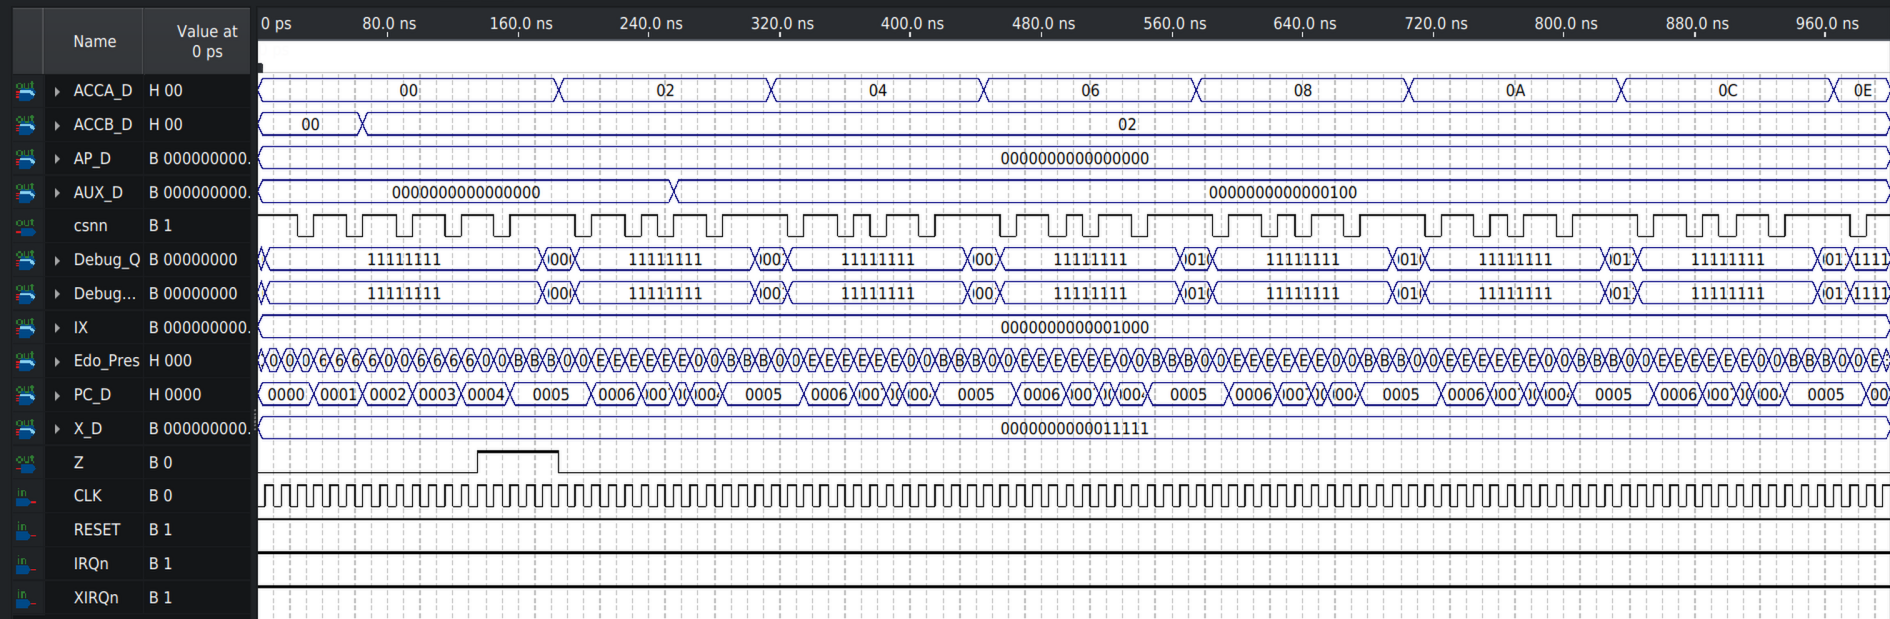
\includegraphics[width=\linewidth]{ejercicio1.png}
\caption{Suma repetitiva con $B=\hx{02}$ y salto a \hx{0004}.}\label{fig:ej1}
\end{figure}
En la Figura~\ref{fig:ej1}, B se carga con \hx{02} y conserva ese valor. A sigue la secuencia \hx{00}, \hx{02}, \hx{04}, \hx{06}, \hx{08}, \hx{0A}, \hx{0C} y \hx{0E}. El PC vuelve a \hx{0004} después de leer el salto y sus operandos. Esto permite ejecutar \texttt{ABA} repetidamente sin volver a cargar $A=0$.

Los intervalos entre cambios de A incluyen la búsqueda, la suma y el salto. Por ello, el resultado no cambia en cada periodo del reloj. La captura verifica el incremento de dos en dos durante la ventana observada; no se alcanzó el desbordamiento del acumulador de 8 bits.

\clearpage
\subsection{Ejercicio 1: salto a la carga de FF}
\begin{figure}[H]\centering
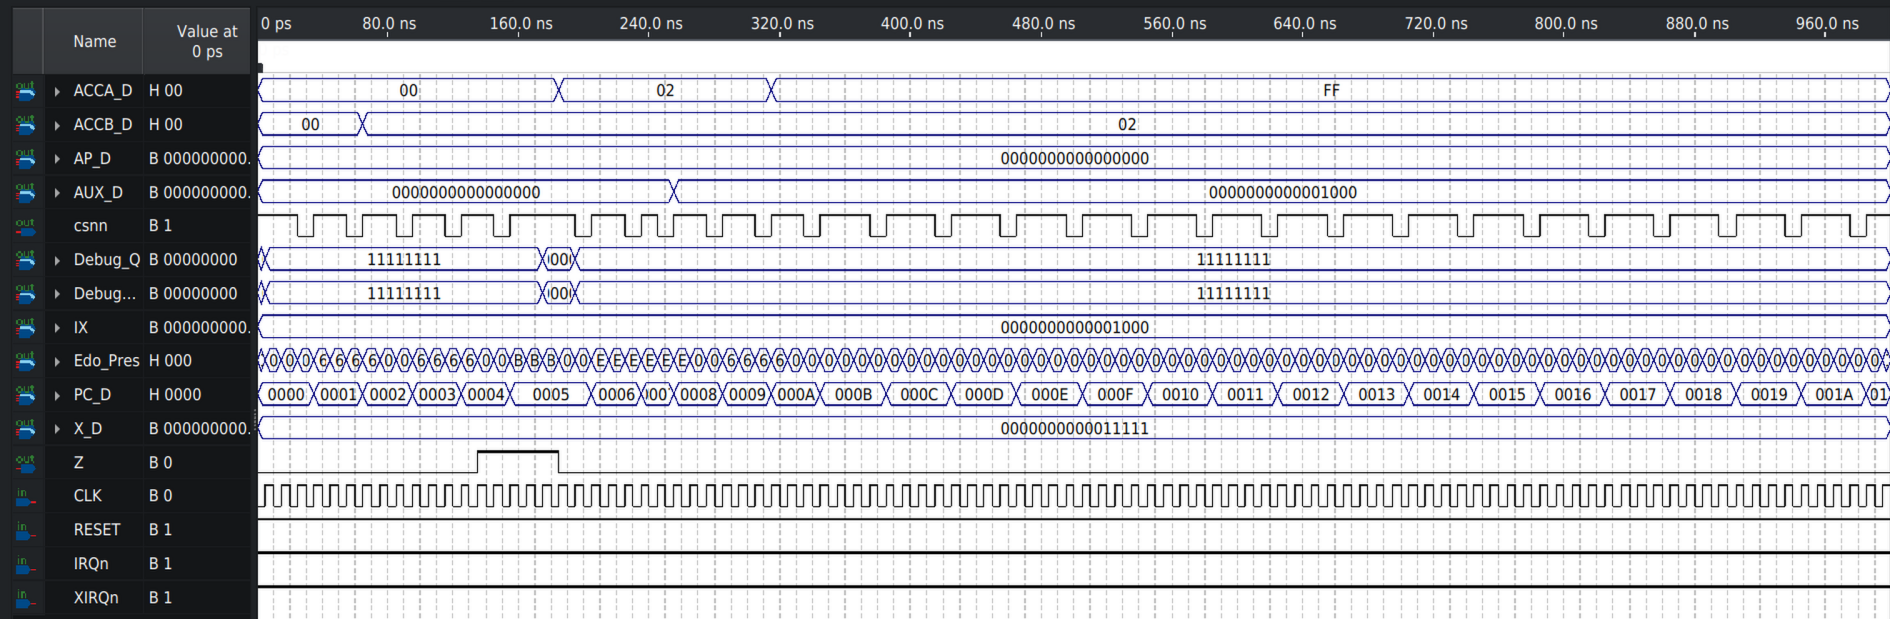
\includegraphics[width=\linewidth]{ejercicio1_ff.png}
\caption{Variante con destino \hx{0008}: después de una suma se carga \hx{FF}.}\label{fig:ej1ff}
\end{figure}
En la Figura~\ref{fig:ej1ff}, A pasa de \hx{00} a \hx{02} y después a \hx{FF}; B permanece en \hx{02}. El destino \hx{0008} impide regresar a la suma y permite ejecutar la carga inmediata ubicada en las posiciones 8 y 9.

Después de esta carga, el PC continúa por la región inicializada con ceros. La permanencia de A en \hx{FF} no corresponde a una instrucción de alto: no se programó un bucle final en esta variante. El resultado permite comprobar el destino del salto y la carga del operando.

\clearpage
\subsection{Ejercicio 2: acumuladores iguales}
\begin{figure}[H]\centering
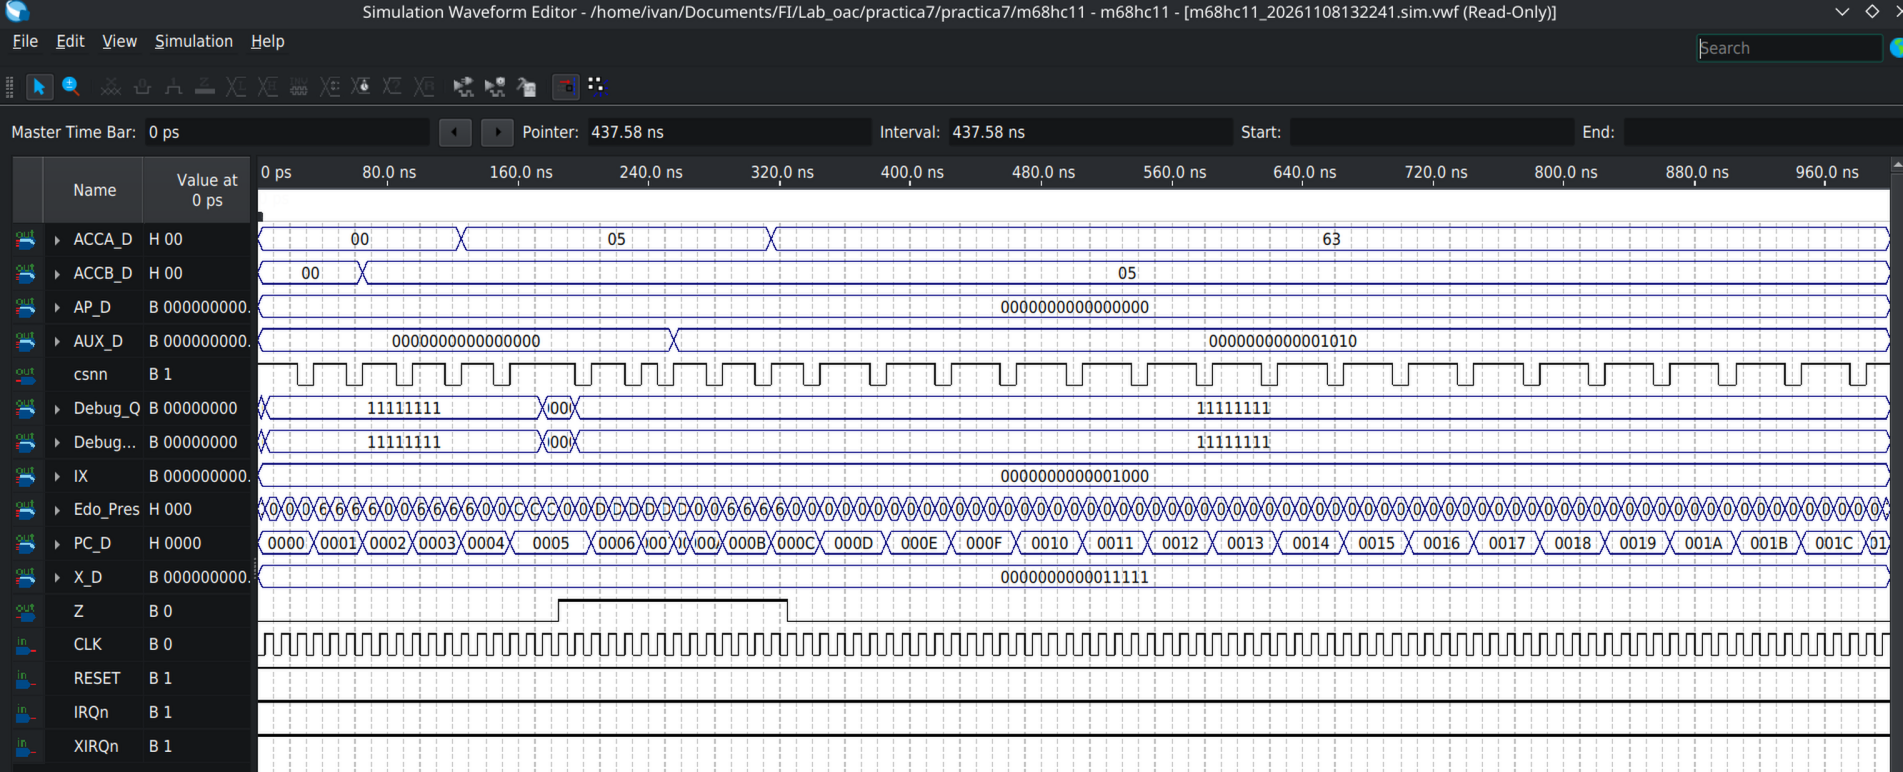
\includegraphics[width=\linewidth,trim=0 0 0 105,clip]{ejercicio_2_iguales.png}
\caption{Comparación de $A=\hx{05}$ y $B=\hx{05}$: se omite la carga de \hx{48}.}\label{fig:ej2igual}
\end{figure}
En la Figura~\ref{fig:ej2igual}, ambos acumuladores reciben \hx{05}. Después de la comparación, $Z$ toma el valor uno y \texttt{JE} conduce al programa a \hx{000A}. A cambia directamente de \hx{05} a \hx{63}; no aparece \hx{48}. Se comprueba que el salto se toma cuando los operandos son iguales.

La bandera $Z$ vuelve a cambiar después de cargar \hx{63}, porque esa instrucción también actualiza las banderas. La condición de igualdad debe revisarse entre \texttt{CMP} y \texttt{JE}, en lugar de usar únicamente el valor final de $Z$.

\clearpage
\subsection{Ejercicio 2: acumuladores diferentes}
\begin{figure}[H]\centering
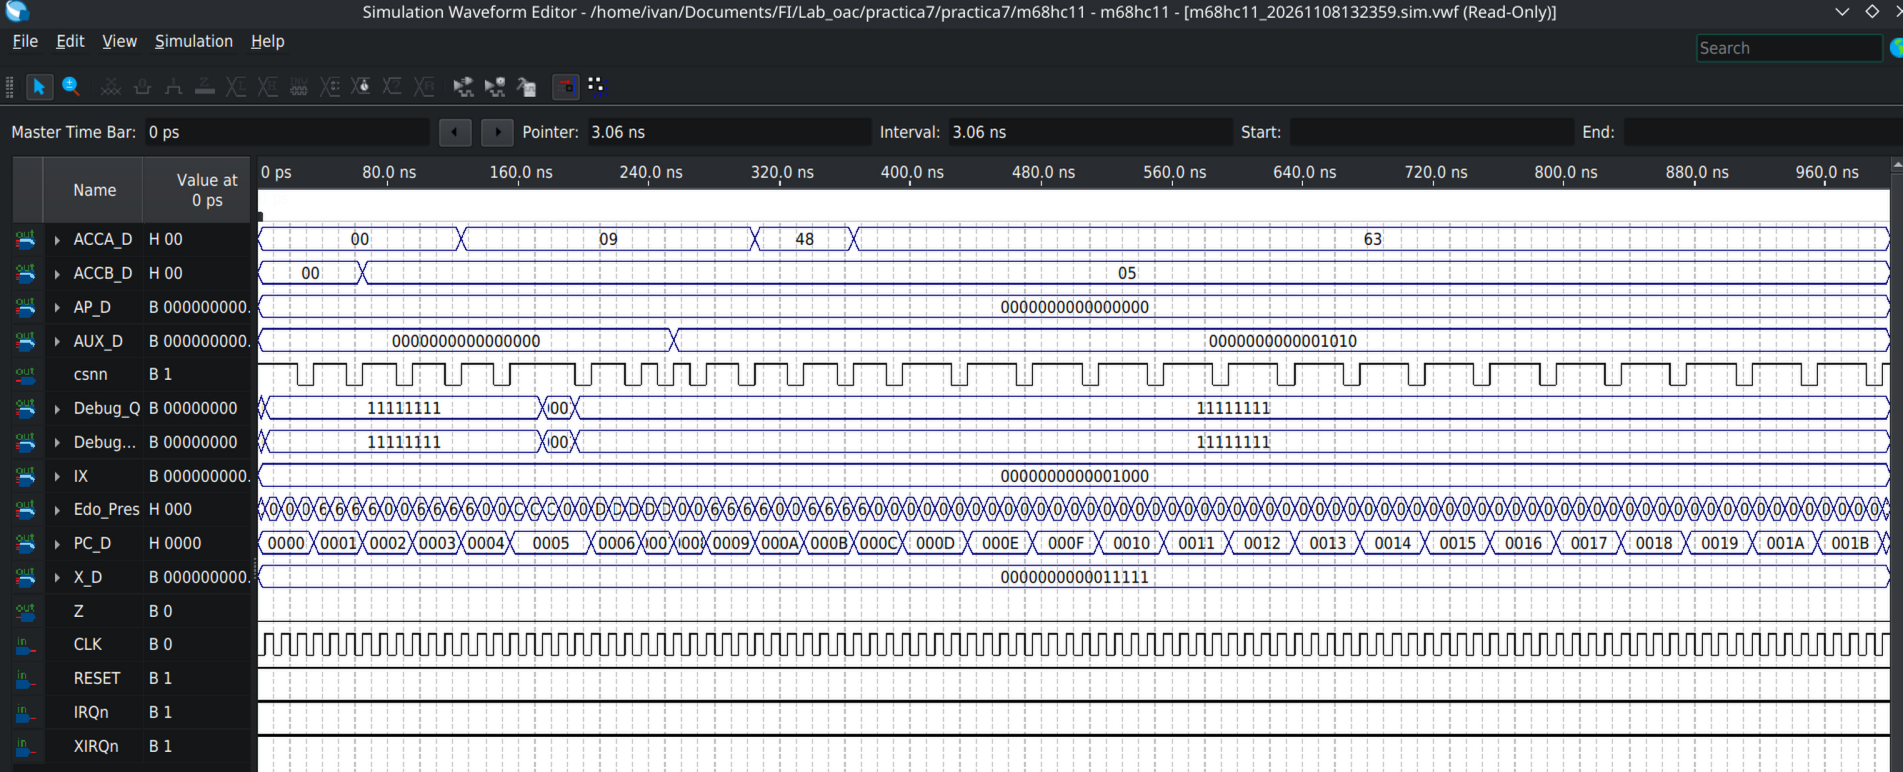
\includegraphics[width=\linewidth,trim=0 0 0 105,clip]{ejercicio_2_diferentes.png}
\caption{Comparación de $A=\hx{09}$ y $B=\hx{05}$: A pasa por \hx{48} y termina en \hx{63}.}\label{fig:ej2dif}
\end{figure}
En la Figura~\ref{fig:ej2dif}, B conserva \hx{05} y A se carga con \hx{09}. La comparación deja $Z=0$, de modo que no se toma el salto a \hx{000A}. Se ejecuta primero la carga de \hx{48} y luego la de \hx{63}, en concordancia con el Listado~\ref{lst:ej2}.

La diferencia respecto a la prueba anterior es el valor intermedio \hx{48} y el recorrido por las posiciones 8 y 9. El valor final \hx{63} es común a ambas pruebas; observarlo de manera aislada no permite decidir si el salto condicional funcionó.

\clearpage
\subsection{Ejercicio 3: variables iguales}
\begin{figure}[H]\centering
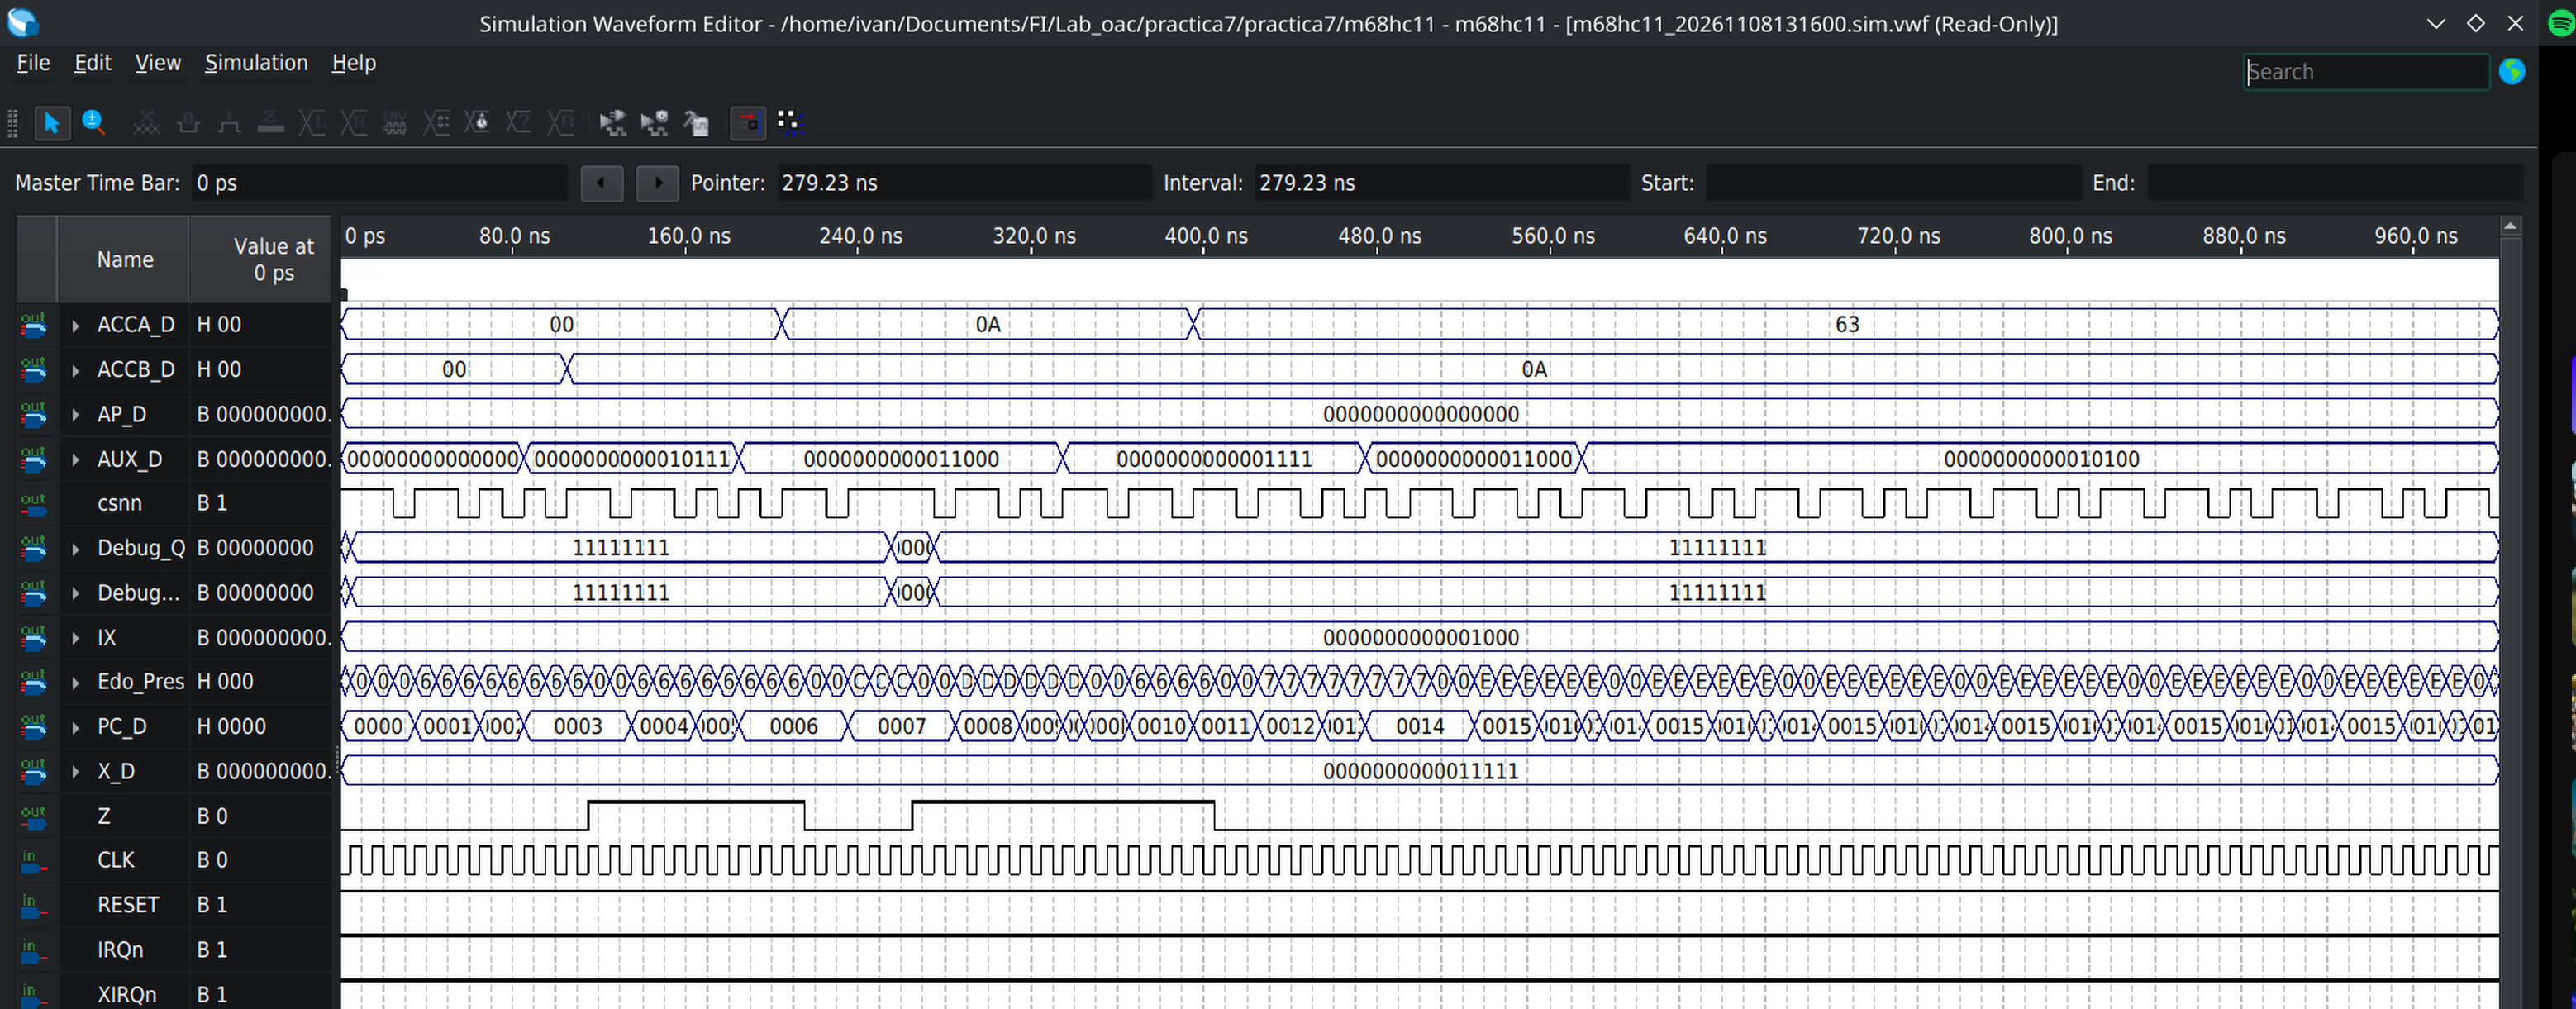
\includegraphics[width=\linewidth,trim=0 0 0 150,clip]{ejercico_3_iguales.png}
\caption{Lectura de \hx{0A} desde ambas variables y salto a la carga común de \hx{63}.}\label{fig:ej3igual}
\end{figure}
En la Figura~\ref{fig:ej3igual}, ambos acumuladores se cargan con \hx{0A} mediante acceso extendido. La comparación activa $Z$ y se omite la ruta que carga y almacena \hx{48}. A cambia de \hx{0A} a \hx{63}; B mantiene \hx{0A}. Al final, el PC recorre repetidamente el \texttt{JMP} situado en \hx{0014}.

El recorrido es consistente con la ejecución de \texttt{STAA} para escribir \hx{63} en \hx{0018}. La captura no muestra directamente el contenido interno de la RAM: el dato escrito se deduce del acumulador y de la secuencia de instrucciones, sin una lectura posterior de verificación.

\clearpage
\subsection{Ejercicio 3: variables diferentes}
\begin{figure}[H]\centering
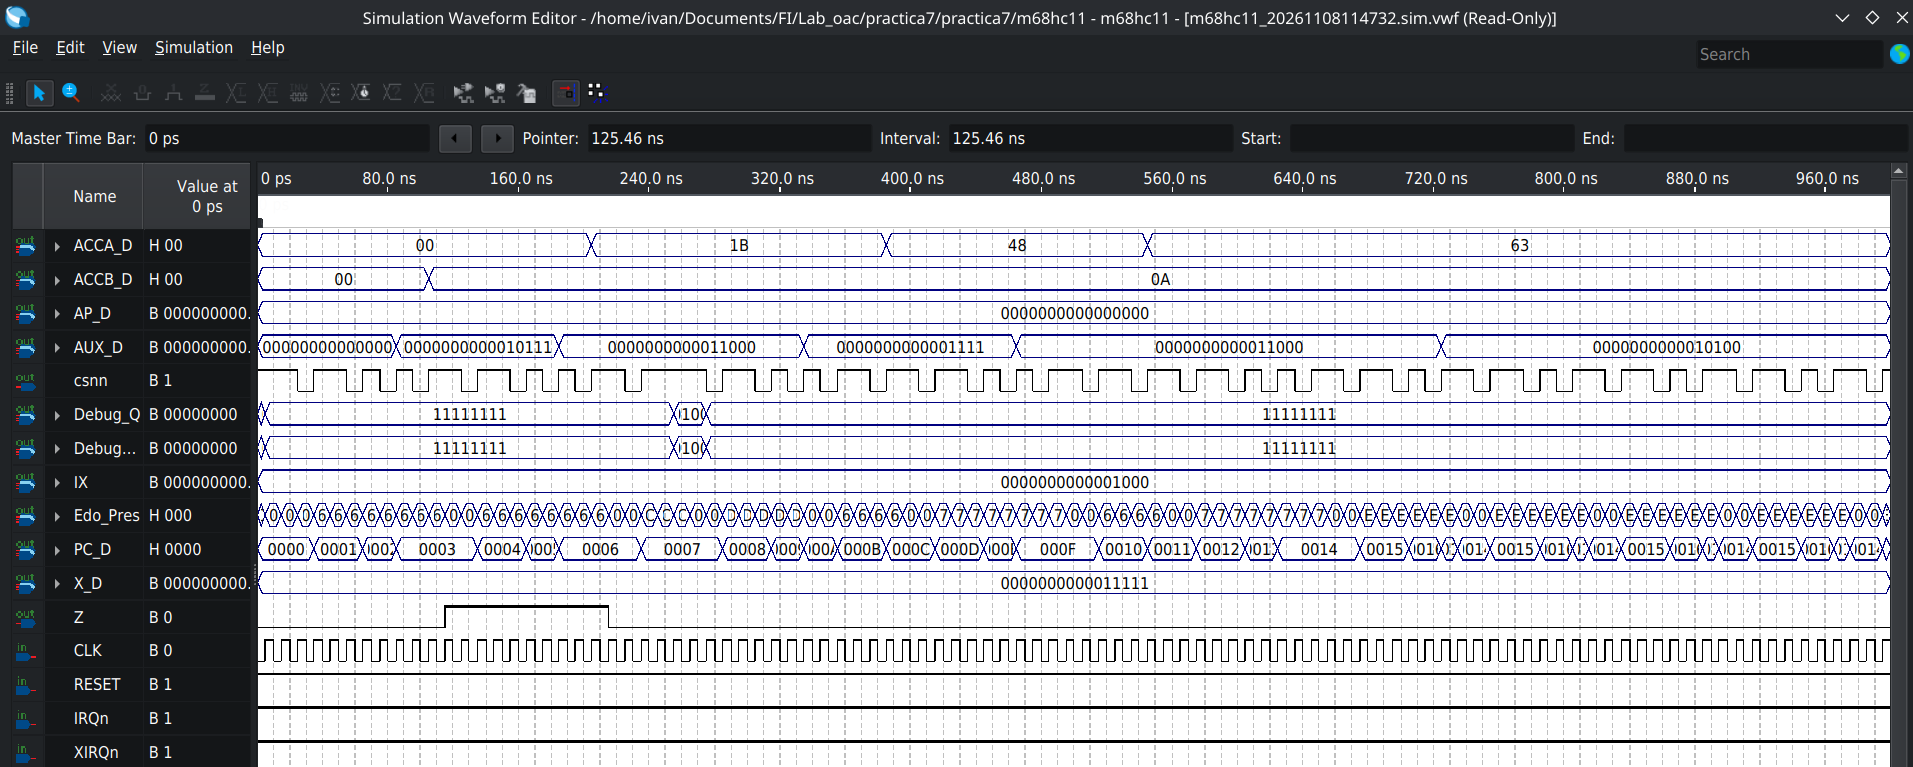
\includegraphics[width=\linewidth,trim=0 0 0 105,clip]{ejercico_3_diferentes.png}
\caption{Lectura de $B=\hx{0A}$ y $A=\hx{1B}$, seguida por las cargas de \hx{48} y \hx{63}.}\label{fig:ej3dif}
\end{figure}
En la Figura~\ref{fig:ej3dif}, \texttt{LDAB} obtiene \hx{0A} de \hx{0017} y \texttt{LDAA} obtiene \hx{1B} de \hx{0018}. No se cumple la igualdad. Se recorre la ruta que carga \hx{48} y ejecuta \texttt{STAA}; después se carga \hx{63} y se ejecuta el segundo almacenamiento. La secuencia visible en A es \hx{00}, \hx{1B}, \hx{48}, \hx{63}.

El bucle final mantiene el PC alrededor de \hx{0014--0016}, correspondientes al opcode \texttt{JMP} y sus operandos. La evidencia permite seguir la ruta de escritura y el dato en A; la captura no incluye una observación directa de la celda \hx{0018}.
\end{landscape}
\restoregeometry

\section{Discusión de resultados}
\begin{table}[H]\centering\small
\caption{Resultados observados en las seis pruebas.}
\begin{tabularx}{\linewidth}{l Y Y}
\toprule
Prueba & Secuencia en A & Comprobación principal \\
\midrule
1: suma & \hx{00,02,04,06,08,0A,0C,0E} & Repetición de \texttt{ABA} con $B=\hx{02}$. \\
1: carga de FF & \hx{00,02,FF} & Salto a \hx{0008} y carga inmediata. \\
2: iguales & \hx{00,05,63} & \texttt{JE} omite la carga de \hx{48}. \\
2: diferentes & \hx{00,09,48,63} & Continuación por la ruta intermedia. \\
3: iguales & \hx{00,0A,63} & Lecturas extendidas y omisión de la primera escritura. \\
3: diferentes & \hx{00,1B,48,63} & Lecturas extendidas y recorrido por ambas escrituras. \\
\bottomrule
\end{tabularx}
\end{table}
Las formas de onda muestran la coordinación entre el PC y las microdirecciones. La suma requiere varias transiciones internas antes de actualizar A. Una instrucción extendida debe obtener dos bytes de dirección antes de realizar el acceso o el salto. Esta diferencia explica por qué una instrucción del programa ocupa varios ciclos del secuenciador.

Las pruebas de comparación muestran que una bandera describe el resultado de la operación que la actualizó más recientemente. Después de \texttt{CMP}, $Z$ sirve para decidir el salto; después de una carga puede cambiar. También se observó que dos ejecuciones pueden terminar con el mismo acumulador y haber seguido rutas distintas, como ocurre con \hx{63} en los ejercicios 2 y 3.

El alcance de la comprobación es la simulación funcional. Las imágenes no documentan una implementación física ni una lectura de retorno de la RAM. La referencia anterior incluye un cuarto ejercicio; éste no se presenta como realizado porque los códigos y las capturas disponibles corresponden a los tres ejercicios descritos.

\clearpage
\section{Conclusiones}
\paragraph{Percival Ulises Espinoza Matamoros.}
La práctica permitió relacionar las instrucciones del programa con las operaciones internas del procesador. La hoja de cálculo del profesor fue útil para organizar las señales y revisar las palabras de microprograma antes de colocarlas en VHDL. Al seguir las microdirecciones y los acumuladores, se pudo comprobar cómo una carga, una suma o un salto requieren varios pasos coordinados.

\paragraph{Oscar Iván Montiel Juárez.}
En esta práctica comprendimos la diferencia entre cambiar el programa de la RAM y modificar la memoria de control. También fue necesario comprobar qué archivo utilizaba Quartus, ya que editar otra copia del MIF mantenía los mismos resultados aunque se volviera a compilar. Una vez corregida la ruta, las pruebas mostraron la suma repetitiva, la carga de \hx{FF} y las dos rutas de comparación según $Z$.

\paragraph{Amy Valentina Veraza García.}
Las pruebas con datos iguales y diferentes ayudaron a interpretar \texttt{CMP} y \texttt{JE}. El valor final de A no fue suficiente para distinguir las rutas, porque ambas terminaban en \hx{63}; fue necesario observar el paso por \hx{48}, la bandera y el PC. El direccionamiento extendido permitió relacionar las variables con sus direcciones en RAM y con las instrucciones de carga y almacenamiento.

\begin{thebibliography}{9}
\bibitem{hoja} Cruz Estrada, J. C. \textit{salidas\_68HC11\_CISC-practica7.xlsx}. Material de apoyo del Laboratorio de Organización y Arquitectura de Computadoras. Hojas \texttt{salidas}, \texttt{entradas}, \texttt{LDAB(INM)}, \texttt{LDAA(INM)} y \texttt{fetch}.
\bibitem{diagramas} Laboratorio de Organización y Arquitectura de Computadoras. \textit{Diagramas de direccionamiento inmediato y extendido}. Archivos \texttt{inmediato.pdf} y \texttt{extendido.pdf}, material proporcionado por el profesor.
\bibitem{control} Laboratorio de Organización y Arquitectura de Computadoras. \textit{Líneas de control y arquitectura del procesador 68HC11}. Archivos \texttt{lineas\_de\_control\_update.pdf} y \texttt{68HC11.pdf}, material proporcionado por el profesor.
\bibitem{anterior} Jiménez Treviño, E. C., y Martinez Perez, B. E. \textit{Práctica 7. Procesador CISC 68HC11}. Reporte del semestre 2026-1, 18 de noviembre de 2025. Referencia de organización y ejercicios.
\end{thebibliography}

\clearpage
\appendix
\section{Código de la memoria de control}
El listado incorpora directamente \texttt{code/memory.vhd}. Se omite únicamente el encabezado de comentarios de formato y ejemplos que precede a los estados activos; se conservan la declaración de la entidad y todas las rutinas implementadas. La numeración corresponde al listado mostrado.
\lstinputlisting[style=estiloVHDL,basicstyle=\ttfamily\fontsize{7}{8.5}\selectfont,
 linerange={1-16,27-113},caption={Memoria de microprograma de la práctica.},label={lst:memoria}]{code/memory.vhd}
\end{document}
